\section{The IIM for the 1D heat equation with moving interface}

In this section we solve the heat equation with a moving interface using the IIM to modify some simple finite difference schemes.

We are solving the heat equation

\begin{equation}
    \frac{\partial u}{\partial t} = \kappa \frac{\partial^2 u}{\partial x^2}
\end{equation}

with $u=u(x,t)$ on $x \in [0,1]$, $t > 0$ and $\kappa > 0$, and with initial and boundary conditions

\begin{equation}
    u(x,0) = U_0(x), \qquad u(0,t) = A, \qquad u(1,t) = B,
\end{equation}

and $\alpha (t) \in [0,1]$ the location of the interface.

We also have jump conditions

\begin{eqnarray}
    [u]_\alpha  =  u^+(\alpha) - u^-(\alpha), \\
    \left[\frac{\partial u}{\partial x}\right]_\alpha  =  \frac{\partial u}{\partial x}^+(\alpha) - \frac{\partial u}{\partial x}^-(\alpha), \\
    \left[\frac{\partial^2 u}{\partial x^2}\right]_\alpha  =  \frac{\partial^2 u}{\partial x^2}^+(\alpha) - \frac{\partial^2 u}{\partial x^2}^-(\alpha). 
\end{eqnarray}

\subsection{Solving for initial condition of two error functions}

The problem we consider is that where the initial condition is 
\begin{equation}
    U_0(x) = \left\{
        \begin{array}{lr}
            \operatorname{Erfc}(\frac{x}{\sqrt{t_0}}) & : x \leq \alpha(t_0) \\
            2 \operatorname{Erfc}(\frac{1-x}{\sqrt{t_0}}) & : x > \alpha(t_0)
        \end{array}
    \right.
\end{equation}

where $\operatorname{Erfc}(z)$ is the complementary error function and with $\kappa = \frac{1}{4}$, $u(0,t) = 1$, $u(1,t) = \frac{1}{2}$ and $\alpha(t)$ is the function which satisfies

\begin{equation}
    \operatorname{Erfc}\left(\frac{\alpha(t)}{\sqrt{t}}\right) = 2 \operatorname{Erfc}\left(\frac{1-\alpha(t)}{\sqrt{t}}\right)
\end{equation}

which must be determined numerically.

The exact solution to this problem is
\begin{equation}
    u(x,t) =  \left\{
    \begin{array}{lr}
        \operatorname{Erfc}(\frac{x}{\sqrt{t}}) & : x \leq \alpha(t) \\
        2 \operatorname{Erfc}(\frac{1-x}{\sqrt{t}}) & : x > \alpha(t)
        \end{array}
    \right.
\end{equation}

We wish to solve this problem approximately using the various methods mentioned in the previous section combined with various discretisation schemes.

For all the schemes, let

\begin{equation}
    x_i = i \Delta x, i = 0, 1, 2, \ldots, N \qquad t_k = k \Delta t, k = 0, 1, 2, \ldots
\end{equation}

and 

\begin{equation}
    u_i^k \approx u(x_i,t_k)
\end{equation}

We now consider a simple example of the use of the IIM to solve a problem where the exact solution is known.
Although the problem is somewhat contrived, knowledge of the solution allows us to evaluation the accuracy of the approximate solutions.

\subsubsection{The forward difference method}

The forward difference method is an explicit method accurate to $\mathcal{O}(\Delta x^2)$ in space and $\mathcal{O}(\Delta t)$ in time, with

\begin{equation}
    \frac{u_i^{k+1} - u_i^k}{\Delta t} = \kappa \frac{u_{i-1}^k - 2 u_i^k + u_{i+1}^k}{\Delta x^2}
\end{equation}

at points away from the interface.
At points adjacent to the interface we modify the finite difference schemes using the Li and Ito method, the undetermined time coefficient method and the Russell and Wang method.

All three methods perform fairly well.
Their errors are of the expected magnitude and are stable over the same range of $\Delta t$ and $\Delta x$ values as for continuous problems.

The only anomalous results is that both the Li and Ito method and the undetermined time coefficient methods do not show monotonic error behavior.
Instead, their error seems to oscillate with no obvious pattern, although it does tend to increase leading up to an irregular timestep before being corrected once the time correction occurs.

\subsubsection{The backwards difference method}

The backwards difference method is an implicit method accurate to $\mathcal{O}(\Delta x^2)$ in space and $\mathcal{O}(\Delta t)$ in time, with

\begin{equation}
    \frac{u_i^{k+1} - u_i^k}{\Delta t} = \kappa \frac{u_{i-1}^{k+1} - 2 u_i^{k+1} + u_{i+1}^{k+1}}{\Delta x^2}
\end{equation}

at points away from the interface.
At points adjacent to the interface we modify the finite difference scheme using the three methods.

Again, all methods perform well.
The errors are of the correct magnitude, but the oscillations that were present for the forward difference method are still present for the Li and Ito and undetermined time coefficient methods.

\subsubsection{The Crank-Nicolson method}

The Crank-Nicolson method is an implicit method which is accurate to $\mathcal{O}(\Delta x^2)$ in space and $\mathcal{O}(\Delta t^2)$ in time, with

\begin{equation}
    \frac{u_i^{k+1} - u_i^k}{\Delta t} = \frac{\kappa}{2}\left(\frac{u_{i-1}^k - 2 u_i^k + u_{i+1}^k}{\Delta x^2} + \frac{u_{i-1}^{k+1} - 2 u_i^{k+1} + u_{i+1}^{k+1}}{\Delta x^2}\right)
\end{equation}

For this method, the Russell and Wang method behaves with the correct error magnitude, however the other two methods do not.

Both the Li and Ito and undetermined time coefficient methods develop large errors near the interface, indicating that they are not correcting sufficiently for the discontinuity as shown in figure \ref{fig:LiItoHeat}

\begin{figure}[p]
    \centering
    \begin{subfigure}[b]{0.85\textwidth}
        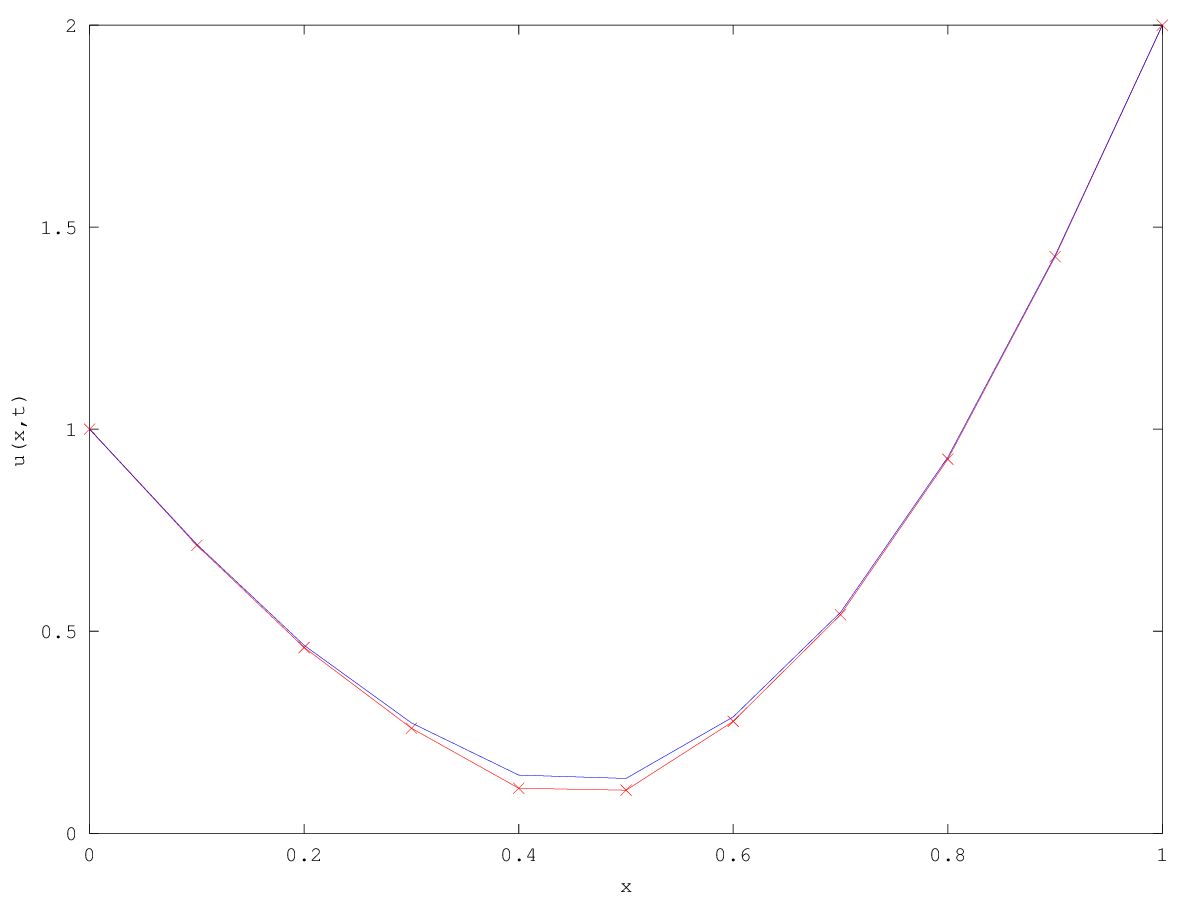
\includegraphics[width=\textwidth]{diagrams/LiItoSmallt}
        \caption{$t=0.15$}
    \end{subfigure}
    \begin{subfigure}[b]{0.85\textwidth}
        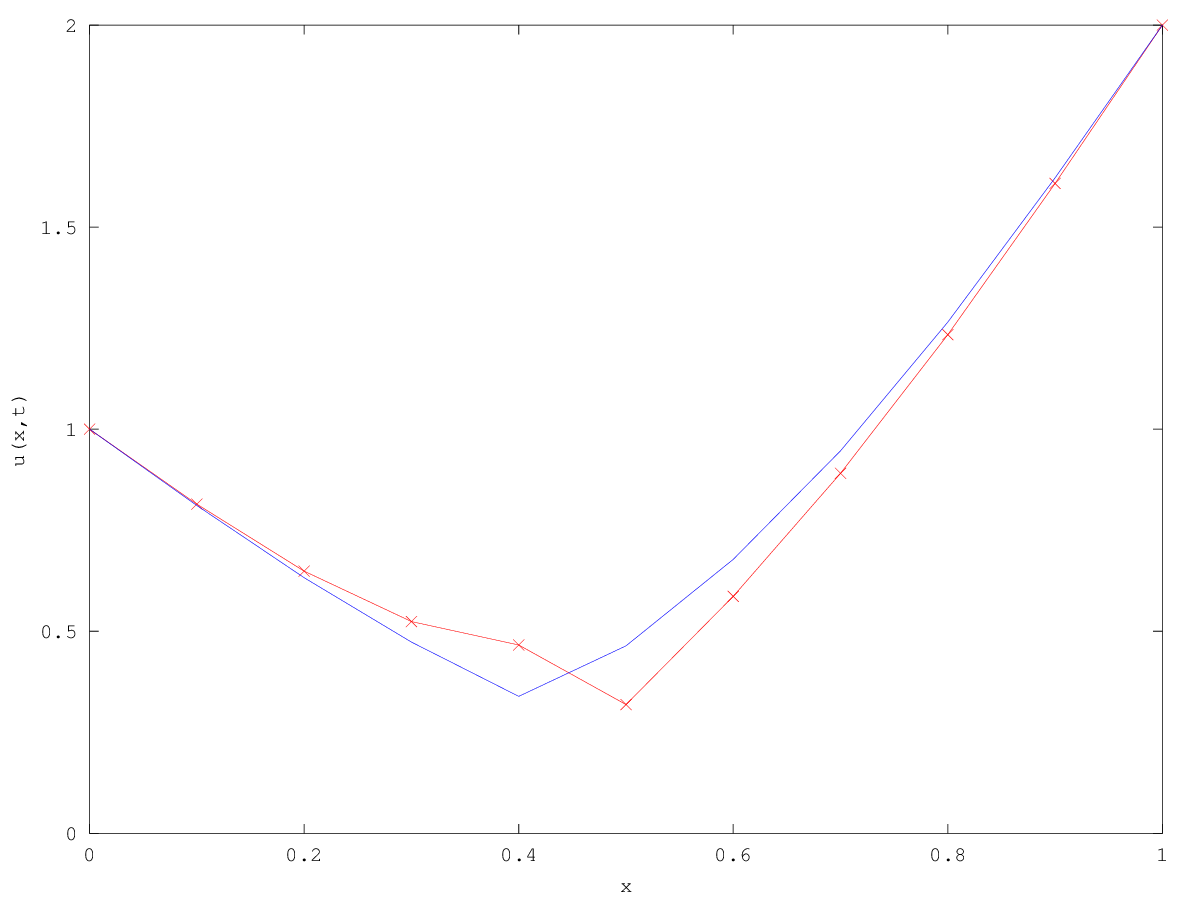
\includegraphics[width=\textwidth]{diagrams/LiItoLarget}
        \caption{$t=0.35$}
    \end{subfigure}
    \caption{Solutions for the Li and Ito method with Crank-Nicolson discretisation for small and large values of $t$.
    The solid line represents the exact solution while the line with $\times$  symbols represents the approximate solution.
    $\Delta x = 0.1$, $\Delta t = 0.01$, $t_0 = 0.1$.}
    \label{fig:LiItoHeat}
\end{figure}
